% Chapter 4: Martingale Inequalities and Convergence
% Based on Basic Stochastic Processes

\chapter{Martingale Inequalities and Convergence}
\label{chap:MartingaleInequalitiesConvergence}

\section{Doob's Martingale Inequalities}
\label{sec:DoobsMartingaleInequalities}

\begin{Proposition}[Doob's maximal inequality]
\label{prop:DoobsMaximalInequality}
Suppose that $\xi_{n}, n \in \mathbb{N}$, is a non-negative submartingale (with respect to a filtration $\mathcal{F}_{n}$). Then for any $\lambda > 0$
\[
\lambda P \left(\max_{k \leq n} \xi_{k} \geq \lambda\right) \leq E \left(\xi_{n} 1_{\left\{\max_{k \leq n} \xi_{k} \geq \lambda \right\}}\right),
\]
where $1_A$ is the characteristic function of a set $A$.
\end{Proposition}

\begin{Proof}
We put $\xi_{n}^{*} = \max_{k\leq n}\xi_{k}$ for brevity. For $\lambda >0$ let us define
\[
\tau = \min \left\{k \leq n: \xi_{k} \geq \lambda \right\},
\]
if there is a $k \leq n$ such that $\xi_k \geq \lambda$, and $\tau = n$ otherwise. Then $\tau$ is a stopping time such that $\tau \leq n$ a.s. Since $\xi_n$ is a submartingale,
\[
E (\xi_{n}) \geq E (\xi_{\tau}).
\]
But
\[
E (\xi_{\tau}) = E \left(\xi_{\tau} 1_{\{\xi_{n}^{*} \geq \lambda \}}\right) + E \left(\xi_{\tau} 1_{\{\xi_{n}^{*} < \lambda \}}\right).
\]
Observe that if $\xi_n^* \geq \lambda$, then $\xi_\tau \geq \lambda$. Moreover, if $\xi_n^* < \lambda$, then $\tau = n$, and so $\xi_\tau = \xi_n$. Therefore
\[
E (\xi_{n}) \geq E (\xi_{\tau}) \geq \lambda P (\xi_{n}^{*} \geq \lambda) + E (\xi_{n} 1_{\{\xi_{n}^{*} < \lambda \}}),
\]
It follows that
\[
\lambda P \left(\xi_{n}^{*} \geq \lambda\right) \leq E \left(\xi_{n}\right) - E \left(\xi_{n} 1_{\{\xi_{n}^{*} < \lambda \}}\right) = E \left(\xi_{n} 1_{\{\xi_{n}^{*} \geq \lambda \}}\right),
\]
completing the proof. \qed
\end{Proof}

\begin{Theorem}[Doob's maximal $L^2$ inequality]
\label{th:DoobsMaximalL2Inequality}
If $\xi_{n}, n \in \mathbb{N}$, is a non-negative square integrable submartingale (with respect to a filtration $\mathcal{F}_{n}$), then
\[
E \left| \max_{k \leq n} \xi_{k} \right|^{2} \leq 4 E | \xi_{n} |^{2}. \tag{4.2}
\]
\end{Theorem}

\begin{Proof}
Put $\xi_{n}^{*} = \max_{k\leq n}\xi_{k}$. By Exercise 1.9, Proposition \ref{prop:DoobsMaximalInequality}, the Fubini theorem and finally the Cauchy-Schwarz inequality
\[
\begin{array}{l}
E \left| \xi_{n}^{*} \right|^{2} = 2 \int_{0}^{\infty} t P \left(\xi_{n}^{*} > t\right) dt \leq 2 \int_{0}^{\infty} E \left(\xi_{n} 1_{\left\{\xi_{n}^{*} \geq t \right\}}\right) dt \\
= 2 \int_{0}^{\infty} \left(\int_{\left\{\xi_{n}^{*} \geq t \right\}} \xi_{n} dP\right) dt = 2 \int_{\Omega} \xi_{n} \left(\int_{0}^{\xi_{n}^{*}} dt\right) dP \\
= 2 \int_{\Omega} \xi_{n} \xi_{n}^{*} dP = 2 E (\xi_{n} \xi_{n}^{*}) \leq 2 (E | \xi_{n} |^{2})^{1/2} (E | \xi_{n}^{*} |^{2})^{1/2}.
\end{array}
\]
Dividing by $\left(E|\xi_n^*|^2\right)^{1/2}$, we get (4.2).
\qed
\end{Proof}

The proof of Doob's Convergence Theorem in the next section hinges on an inequality involving the number of upcrossings.

\begin{Definition}
\label{def:UpcrossingsStrategy}
Given an adapted sequence of random variables $\xi_1, \xi_2, \ldots$ and two real numbers $a < b$, we define a gambling strategy $\alpha_1, \alpha_2, \ldots$ by putting
\[
\alpha_{1} = 0
\]
and for $n = 1,2,\ldots$
\[
\alpha_{n + 1} = \left\{ \begin{array}{ll}
1 & \text{if } \alpha_{n} = 0 \text{ and } \xi_{n} < a, \\
1 & \text{if } \alpha_{n} = 1 \text{ and } \xi_{n} \leq b, \\
0 & \text{otherwise.}
\end{array} \right.
\]
It will be called the \textbf{upcrossings strategy}. Each $k = 1,2,\ldots$ such that $\alpha_{k} = 1$ and $\alpha_{k + 1} = 0$ will be called an upcrossing of the interval $[a,b]$. The upcrossings form a (finite or infinite) increasing sequence
\[
u_{1} < u_{2} < \dots .
\]
The number of upcrossings made up to time $n$, that is, the largest $k$ such that $u_{k} \leq n$ will be denoted by $U_{n}[a,b]$ (we put $U_{n}[a,b] = 0$ if no such $k$ exists).
\end{Definition}

The meaning of the above definition is this. Initially, we refrain from playing the game and wait until $\xi_{n}$ becomes less than $a$. As soon as this happens, we start playing unit stakes at each round of the game and continue until $\xi_{n}$ becomes greater than $b$. At this stage we refrain from playing again, wait until $\xi_{n}$ becomes less than $a$, and so on. The strategy $\alpha_{n}$ is defined in such a way that $\alpha_{n}=0$ whenever we refrain from playing the $n$-th game, and $\alpha_{n}=1$ otherwise. During each run of consecutive games with $\alpha_{n}=1$ the process $\xi_{n}$ crosses the interval $[a,b]$, starting below $a$ and finishing above $b$. This is what is meant by an upcrossing. Observe that each upcrossing will increase our total winnings by at least $b-a$. For convenience, we identify each upcrossing with its last step $k$, such that $\alpha_{k}=1$ and $\alpha_{k+1}=0$. A typical sample path of the upcrossings strategy is shown in Figure \ref{fig:upcrossings}.

\begin{figure}[H]
\centering
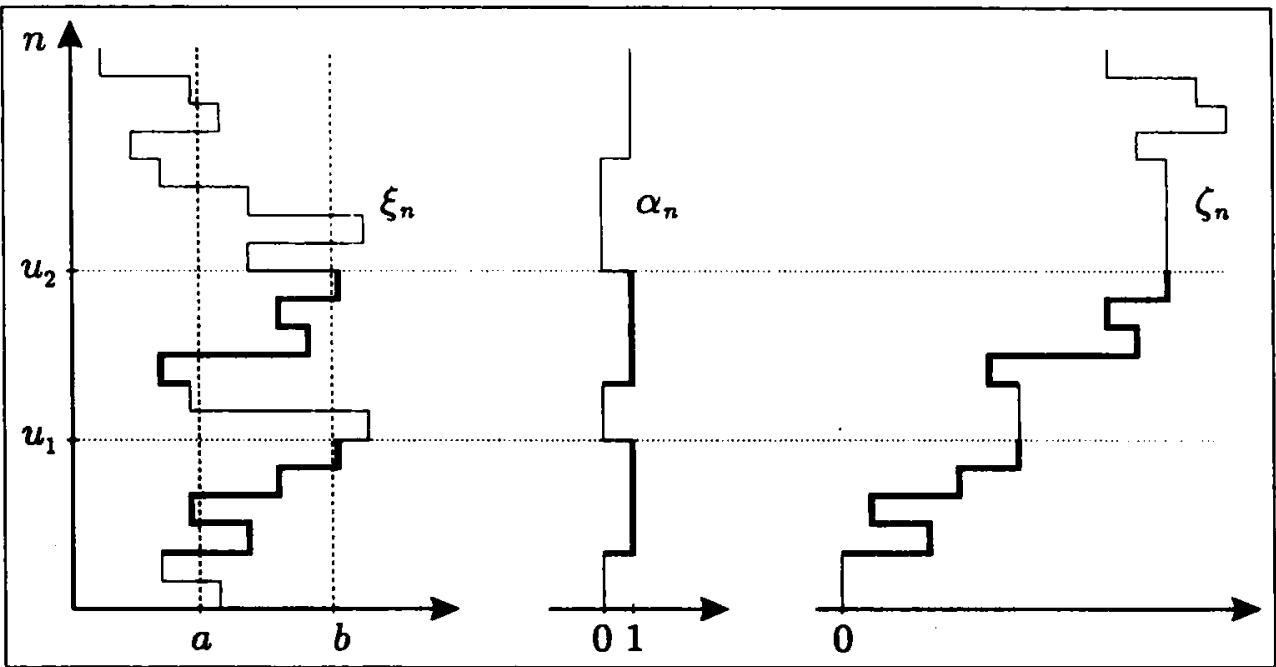
\includegraphics[width=0.8\textwidth]{images/chunk1_6bcc94df728b1e3945dd4adb9d0a2e10494066ffc8c1e84d4b382375949685aa.jpg}
\caption{Typical paths of $\xi_{n}$, $\alpha_{n}$ and $\zeta_{n}$; upcrossings are indicated by bold lines}
\label{fig:upcrossings}
\end{figure}

\begin{Exercise}
\label{ex:UpcrossingsStrategyIsGambling}
Verify that the upcrossings strategy $\alpha_{n}$ is indeed a gambling strategy.

\textit{Hint}: You want to prove that $\alpha_{n}$ is $\mathcal{F}_{n-1}$-measurable for each $n$. Since the upcrossings strategy is defined by induction, a proof by induction on $n$ may be your best bet.
\end{Exercise}

\begin{Solution}
\label{sol:Exercise41}
Because $\alpha_{1} = 0$ is constant, it is $\mathcal{F}_0 = \{\emptyset, \Omega\}$-measurable. Suppose that $\alpha_{n}$ is $\mathcal{F}_{n-1}$-measurable for some $n = 1, 2, \ldots$. Then
\[
\left\{\alpha_{n} = 0, \xi_{n} < a \right\} \cup \left\{\alpha_{n} = 1, \xi_{n} \leq b \right\} \in \mathcal{F}_{n}
\]
because $\mathcal{F}_{n - 1}\subset \mathcal{F}_n$ and $\xi_{n}$ is $\mathcal{F}_n$-measurable. This means that
\[
\alpha_{n + 1} = 1_{\{\alpha_{n} = 0, \xi_{n} < a \} \cup \{\alpha_{n} = 1, \xi_{n} \leq b \}}
\]
is $\mathcal{F}_n$-measurable. By induction it follows that $\alpha_n$ is $\mathcal{F}_{n-1}$-measurable for each $n = 1, 2, \ldots$, so $\alpha_1, \alpha_2, \ldots$ is a gambling strategy.
\end{Solution}

\begin{Lemma}[Upcrossings Inequality]
\label{lma:UpcrossingsInequality}
If $\xi_1, \xi_2, \ldots$ is a supermartingale and $a < b$, then
\[
(b - a) E (U_{n}[a, b]) \leq E ((\xi_{n} - a)^{-}).
\]
By $x^{-}$ we denote the negative part of a real number $x$, i.e. $x^{-} = \max \{0, -x\}$.
\end{Lemma}

\begin{Proof}
Let
\[
\zeta_{n} = \alpha_{1} (\xi_{1} - \xi_{0}) + \dots + \alpha_{n} (\xi_{n} - \xi_{n-1})
\]
be the total winnings at step $n = 1,2,\ldots$ if the upcrossings strategy is followed, see Figure \ref{fig:upcrossings}. It will be convenient to put $\zeta_0 = 0$. By Proposition 3.1 (one cannot beat the system using a gambling strategy) $\zeta_n$ is a supermartingale.

Let us fix an $n$ and put $k = U_{n}[a, b]$, so that
\[
0 < u_{1} < u_{2} < \dots < u_{k} \leq n.
\]
Clearly, each upcrossing increases the total winnings by $b - a$,
\[
\zeta_{u_i} - \zeta_{u_{i-1}} \geq b - a
\]
for $i = 1, \ldots, k$. (We put $u_0 = 0$ for simplicity.) Moreover,
\[
\zeta_{n} - \zeta_{u_k} \geq -(\xi_{n} - a)^{-}.
\]
It follows that
\[
\zeta_{n} \geq (b - a) U_{n}[a, b] - (\xi_{n} - a)^{-}.
\]
Taking the expectation on both sides, we get
\[
E \left(\zeta_{n}\right) \geq (b - a) E (U_{n}[a, b]) - E ((\xi_{n} - a)^{-}).
\]
But $\zeta_{n}$ is a supermartingale, so
\[
0 = E (\zeta_{1}) \geq E (\zeta_{n}),
\]
which proves the Upcrossings Inequality. \qed
\end{Proof}

\section{Doob's Martingale Convergence Theorem}
\label{sec:DoobsMartingaleConvergenceTheorem}

\begin{Theorem}[Doob's Martingale Convergence Theorem]
\label{th:DoobsMartingaleConvergenceTheorem}
Suppose that $\xi_1, \xi_2, \ldots$ is a supermartingale (with respect to a filtration $\mathcal{F}_1, \mathcal{F}_2, \ldots$) such that
\[
\sup_{n} E \left(\left| \xi_{n} \right|\right) < \infty .
\]
Then there is an integrable random variable $\xi$ such that
\[
\lim_{n \rightarrow \infty} \xi_{n} = \xi \quad \text{a.s.}
\]
\end{Theorem}

\begin{Remark}
\label{rem:MartingaleConvergenceRemark1}
In particular, the theorem is valid for martingales because every martingale is a supermartingale. It is also valid for submartingales, since $\xi_{n}$ is a submartingale if and only if $-\xi_{n}$ is a supermartingale.
\end{Remark}

\begin{Remark}
\label{rem:MartingaleConvergenceRemark2}
Observe that even though all the $\xi_{n}$ as well as the limit $\xi$ are integrable random variables, it is claimed only that $\xi_{n}$ trends to $\xi$ a.s. Note that no convergence in $L^{1}$ is asserted.
\end{Remark}

\begin{Proof}[Proof of Doob's Martingale Convergence Theorem]
By the Upcrossings Inequality (Lemma \ref{lma:UpcrossingsInequality})
\[
E \left(U_{n}[a, b]\right) \leq \frac{E \left(\left(\xi_{n} - a\right)^{-}\right)}{b - a} \leq \frac{M + |a|}{b - a} < \infty,
\]
where
\[
M = \sup_{n} E (| \xi_{n} |) < \infty .
\]
Since $U_{n}[a,b]$ is a non-decreasing sequence, it follows that
\[
E \left(\lim_{n \rightarrow \infty} U_{n}[a, b]\right) = \lim_{n \rightarrow \infty} E (U_{n}[a, b]) \leq \frac{M + |a|}{b - a} < \infty .
\]
This implies that
\[
P \left\{\lim_{n \rightarrow \infty} U_{n}[a, b] < \infty \right\} = 1
\]
for any $a < b$. Since the set of all pairs of rational numbers $a < b$ is countable, the event
\[
A = \bigcap_{a < b \text{ rational }} \left\{\lim_{n \rightarrow \infty} U_{n}[a, b] < \infty \right\} \tag{4.3}
\]
has probability 1. (The intersection of countably many events has probability 1 if each of these events has probability 1.)

We claim that the sequence $\xi_{n}$ converges a.s. to a limit $\xi$. Consider the set
\[
B = \left\{\lim_{n} \inf \xi_{n} < \lim_{n} \sup \xi_{n} \right\} \subset \Omega
\]
on which the sequence $\xi_{n}$ fails to converge. Then for any $\omega \in B$ there are rational numbers $a, b$ such that
\[
\liminf_{n} \xi_{n}(\omega) < a < b < \limsup_{n} \xi_{n}(\omega),
\]
implying that $\lim_{n\to \infty}U_n[a,b](\omega) = \infty$. This means that $B$ and the event $A$ in (4.3) are disjoint, so $P(B) = 0$, since $P(A) = 1$, which proves the claim.

It remains to show that the limit $\xi$ is an integrable random variable. By Fatou's lemma
\[
\begin{array}{l}
E (| \xi |) = E \left(\lim_{n} \inf | \xi_{n} |\right) \\
\leq \operatorname*{liminf}_{n} E (| \xi_{n} |) \\
< \sup_{n} E (| \xi_{n} |) < \infty .
\end{array}
\]
This completes the proof. \qed
\end{Proof}

\begin{Exercise}
\label{ex:NonNegativeSupermartingaleConvergence}
Show that if $\xi_{n}$ is a non-negative supermartingale, then it converges a.s. to an integrable random variable.

\textit{Hint}: To apply Doob's Theorem all you need to verify is that the sequence $\xi_{n}$ is bounded in $L^{1}$, i.e. the supremum of $E(|\xi_n|)$ is less than $\infty$.
\end{Exercise}

\begin{Solution}
\label{sol:Exercise42}
For a non-negative supermartingale
\[
\sup_{n} E \left(| \xi_{n} |\right) = \sup_{n} E \left(\xi_{n}\right) \leq E \left(\xi_{1}\right) = E \left(| \xi_{1} |\right) < \infty ,
\]
since
\[
E \left(\xi_{n}\right) \leq E \left(\xi_{1}\right)
\]
for each $n = 1,2,\ldots$. Thus Doob's Martingale Convergence Theorem implies that $\xi_{n}$ converges a.s. to an integrable limit.
\end{Solution}

\section{Uniform Integrability and $L^1$ Convergence of Martingales}
\label{sec:UniformIntegrabilityAndL1Convergence}

The conditions of Doob's theorem imply pointwise (a.s.) convergence of martingales. In this section we shall study convergence in $L^1$. To this end we introduce a stronger condition called uniform integrability. Proposition \ref{prop:UniformIntegrabilityNecessary} shows that it is a necessary condition for $L^1$ convergence. In Theorem \ref{th:UniformIntegrabilitySufficient} we prove that uniform integrability is in fact sufficient for a martingale to converge in $L^1$. This enables us to show that each integrable martingale is of the form $E(\xi | \mathcal{F}_n)$. As an application we give a martingale proof of Kolmogorov's 0-1 law.

\begin{Exercise}
\label{ex:IntegrableCharacterization}
Show that a random variable $\xi$ is integrable if and only if for every $\varepsilon > 0$ there exists an $M > 0$ such that
\[
\int_{\{| \xi | > M \}} | \xi | d P < \varepsilon .
\]

\textit{Hint}: Split $\Omega$ into two sets: $\{|\xi| > M\}$ and $\{|\xi| \leq M\}$. The integrals of $|\xi|$ over these sets must add up to $E(|\xi|)$. As $M$ increases, one of the integrals increases, while the other one decreases. Investigate their limits as $M \to \infty$.
\end{Exercise}

\begin{Solution}
\label{sol:Exercise43}
\textbf{Necessity.} Suppose that $\xi$ is integrable. It follows that
\[
P \left\{\left| \xi \right| < \infty \right\} = 1.
\]
The sequence of random variables $|\xi| 1_{\{|\xi|>M\}}$ indexed by $M = 1,2,\ldots$ is monotone and
\[
| \xi | 1_{\{|\xi| > M\}} \searrow 0 \quad \text{as } M \to \infty
\]
on the set $\{|\xi| < \infty\}$, i.e. a.s. By the monotone convergence theorem for integrals
\[
\int_{\{|\xi| > M\}} | \xi | d P \searrow 0 \quad \text{as } M \to \infty .
\]
It follows that for every $\varepsilon > 0$ there exists an $M > 0$ such that
\[
\int_{\{|\xi| > M\}} | \xi | d P < \varepsilon .
\]

\textbf{Sufficiency.} Take $\varepsilon = 1$. There exists an $M > 0$ such that
\[
\int_{\{|\xi| > M\}} | \xi | d P < 1.
\]
Then
\[
\begin{array}{l}
E (| \xi |) = \int_{\Omega} | \xi | d P \\
= \int_{\{|\xi| > M\}} | \xi | d P + \int_{\{|\xi| \leq M\}} | \xi | d P \\
< 1 + M P \{|\xi| \leq M \} \\
\leq 1 + M < \infty .
\end{array}
\]
\end{Solution}

Thus, for any sequence $\xi_{n}$ of integrable random variables and any $\varepsilon > 0$ there is a sequence of numbers $M_{n} > 0$ such that
\[
\int_{\{| \xi_{n} | > M_{n} \}} | \xi_{n} | d P < \varepsilon .
\]
If the $M_{n}$ are independent of $n$, then we say that the sequence $\xi_{n}$ is uniformly integrable.

\begin{Definition}
\label{def:UniformIntegrability}
A sequence $\xi_1, \xi_2, \ldots$ of random variables is called \textbf{uniformly integrable} if for every $\varepsilon > 0$ there exists an $M > 0$ such that
\[
\int_{\{| \xi_{n} | > M \}} | \xi_{n} | d P < \varepsilon
\]
for all $n = 1,2,\ldots$
\end{Definition}

\begin{Exercise}
\label{ex:NonUniformlyIntegrableExample}
Let $\Omega = [0,1]$ with the $\sigma$-field of Borel sets and Lebesgue measure. Take
\[
\xi_{n} = n 1_{(0, \frac{1}{n})}.
\]
Show that the sequence $\xi_1, \xi_2, \ldots$ is not uniformly integrable.

\textit{Hint}: What is the integral of $\xi_{n}$ over $\{\xi_n > M\}$ if $n > M$?
\end{Exercise}

\begin{Solution}
\label{sol:Exercise44}
For any $M > 0$ and any $n > M$ we have
\[
(0, \frac{1}{n}) = \{\xi_{n} > M\},
\]
so
\[
\int_{\{\xi_{n} > M\}} \xi_{n} d P = \int_{(0, \frac{1}{n})} n d P = 1.
\]
This means that there is no $M > 0$ such that for all $n$
\[
\int_{\{\xi_{n} > M\}} \xi_{n} d P < \frac{1}{2}.
\]
The sequence $\xi_{n}$ is not uniformly integrable.
\end{Solution}

\begin{Proposition}
\label{prop:UniformIntegrabilityNecessary}
Uniform integrability is a necessary condition for a sequence $\xi_1, \xi_2, \ldots$ of integrable random variables to converge in $L^1$.
\end{Proposition}

\begin{Lemma}
\label{lma:AbsoluteContinuityOfIntegral}
If $\xi$ is integrable, then for every $\varepsilon > 0$ there is a $\delta > 0$ such that
\[
P (A) < \delta \Longrightarrow \int_{A} | \xi | d P < \varepsilon .
\]
\end{Lemma}

\begin{Proof}[Proof of Lemma \ref{lma:AbsoluteContinuityOfIntegral}]
Let $\varepsilon > 0$. Since $\xi$ is integrable, by Exercise \ref{ex:IntegrableCharacterization} there is an $M > 0$ such that
\[
\int_{\{| \xi | > M \}} | \xi | d P < \frac{\varepsilon}{2}.
\]
Now
\[
\begin{array}{l}
\int_{A} | \xi | d P = \int_{A \cap \{| \xi | \leq M \}} | \xi | d P + \int_{A \cap \{| \xi | > M \}} | \xi | d P \\
\leq \int_{A} M d P + \int_{\{| \xi | > M \}} | \xi | d P \\
< M P (A) + \frac{\varepsilon}{2}.
\end{array}
\]
Let $\delta = \frac{\epsilon}{2M}$. Then
\[
P (A) < \delta \Longrightarrow \int_{A} | \xi | d P < \varepsilon ,
\]
as required. \qed
\end{Proof}

\begin{Exercise}
\label{ex:ConditionalExpectationUniformlyIntegrable}
Let $\xi$ be an integrable random variable and $\mathcal{F}_1, \mathcal{F}_2, \ldots$ a filtration. Show that $E(\xi | \mathcal{F}_n)$ is a uniformly integrable martingale.

\textit{Hint}: Use Lemma \ref{lma:AbsoluteContinuityOfIntegral}.
\end{Exercise}

\begin{Solution}
\label{sol:Exercise45}
In Example 3.4 it was verified that $\xi_{n} = E(\xi|\mathcal{F}_{n})$ is a martingale. Let $\varepsilon > 0$. By Lemma \ref{lma:AbsoluteContinuityOfIntegral} there is a $\delta > 0$ such that
\[
P (A) < \delta \Longrightarrow \int_{A} | \xi | d P < \varepsilon .
\]
By Jensen's inequality $|\xi_n| \leq E(|\xi||\mathcal{F}_n)$ a.s., so
\[
E (| \xi |) \geq E (| \xi_{n} |) \geq \int_{\{|\xi_{n}| \geq M\}} | \xi_{n} | d P \geq M P \{|\xi_{n}| > M\}.
\]
If we take $M > E(|\xi|) / \delta$, then
\[
P \{|\xi_{n}| > M\} < \delta .
\]
Since $\{|\xi_n| > M\} \in \mathcal{F}_n$, it follows that
\[
\int_{\{|\xi_{n}| > M\}} | \xi_{n} | d P \leq \int_{\{|\xi_{n}| > M\}} E (| \xi | | \mathcal{F}_{n}) d P = \int_{\{|\xi_{n}| > M\}} | \xi | d P < \varepsilon ,
\]
proving that $\xi_{n} = E(\xi |\mathcal{F}_{n})$ is a uniformly integrable sequence.
\end{Solution}

\begin{Proof}[Proof of Proposition \ref{prop:UniformIntegrabilityNecessary}]
Suppose that $\xi_{n} \to \xi$ in $L^{1}$, i.e. $E|\xi_{n} - \xi| \to 0$. We take any $\varepsilon > 0$. There is an integer $N$ such that
\[
n \geq N \Longrightarrow E | \xi_{n} - \xi | < \frac{\varepsilon}{2}.
\]
By Lemma \ref{lma:AbsoluteContinuityOfIntegral} there is a $\delta > 0$ such that
\[
P (A) < \delta \Longrightarrow \int_{A} | \xi | d P < \frac{\varepsilon}{2}.
\]
Taking a smaller $\delta > 0$ if necessary, we also have
\[
P (A) < \delta \Longrightarrow \int_{A} | \xi_{n} | d P < \varepsilon \quad \text{for } n = 1, \dots , N.
\]
We claim that there is an $M > 0$ such that
\[
P \left\{\left| \xi_{n} \right| > M \right\} < \delta
\]
for all $n$. Indeed, since
\[
E \left(| \xi_{n} |\right) \geq \int_{\{| \xi_{n} | > M \}} | \xi_{n} | d P \geq M P \left\{| \xi_{n} | > M \right\},
\]
it suffices to take
\[
M = \frac{1}{\delta} \sup_{n} E (| \xi_{n} |).
\]
(Because the sequence $\xi_{n}$ converges in $L^1$, it is bounded in $L^1$, so the supremum is $< \infty$.)

Now, since $P\{|\xi_n| > M\} < \delta$,
\[
\begin{array}{l}
\int_{\{| \xi_{n} | > M \}} | \xi_{n} | d P \leq \int_{\{| \xi_{n} | > M \}} | \xi | d P + \int_{\{| \xi_{n} | > M \}} | \xi_{n} - \xi | d P \\
\leq \int_{\{| \xi_{n} | > M \}} | \xi | d P + E (| \xi_{n} - \xi |) \\
< \frac{\varepsilon}{2} + \frac{\varepsilon}{2} = \varepsilon .
\end{array}
\]
for any $n > N$ and
\[
\int_{\{| \xi_{n} | > M \}} | \xi_{n} | d P < \varepsilon
\]
for any $n = 1, \ldots, N$, completing the proof.
\end{Proof}

\begin{Exercise}
\label{ex:UniformlyIntegrableBoundedInL1}
Show that a uniformly integrable sequence of random variables is bounded in $L^1$, i.e.
\[
\sup_{n} E \left(\left| \xi_{n} \right|\right) < \infty .
\]

\textit{Hint}: Write $E(|\xi_n|)$ as the sum of the integrals of $|\xi_n|$ over $\{|\xi_n| > M\}$ and $\{|\xi_n| \leq M\}$.
\end{Exercise}

\begin{Solution}
\label{sol:Exercise46}
Because $\xi_{n}$ is a uniformly integrable sequence, there is an $M > 0$ such that for all $n$
\[
\int_{\{|\xi_{n}| > M\}} | \xi_{n} | d P < 1.
\]
It follows that
\[
\begin{array}{l}
E \left(\left| \xi_{n} \right|\right) = \int_{\left\{\left| \xi_{n} \right| > M \right\}} \left| \xi_{n} \right| d P + \int_{\left\{\left| \xi_{n} \right| \leq M \right\}} \left| \xi_{n} \right| d P \\
< 1 + M P \left\{\left| \xi_{n} \right| \leq M \right\} \\
< 1 + M < \infty
\end{array}
\]
for all $n$, proving that $\xi_{n}$ is a bounded sequence in $L^{1}$.
\end{Solution}

Exercise \ref{ex:UniformlyIntegrableBoundedInL1} implies that each uniformly integrable martingale satisfies the conditions of Doob's theorem. Therefore it converges a.s. to an integrable random variable. We shall show that in fact it converges in $L^1$.

\begin{Theorem}
\label{th:UniformIntegrabilitySufficient}
Every uniformly integrable supermartingale (submartingale) $\xi_{n}$ converges in $L^1$.
\end{Theorem}

\begin{Proof}
By Exercise \ref{ex:UniformlyIntegrableBoundedInL1} the sequence $\xi_{n}$ is bounded in $L^1$, so it satisfies the conditions of Theorem \ref{th:DoobsMartingaleConvergenceTheorem} (Doob's Martingale Convergence Theorem). Therefore, there is an integrable random variable $\xi$ such that $\xi_{n} \to \xi$ a.s. We can assume without loss of generality that $\xi = 0$ (since $\xi_{n} - \xi$ can be taken in place of $\xi_{n}$). That is to say,
\[
P \left\{\lim_{n} \xi_{n} = 0 \right\} = 1.
\]
It follows that $\xi_{n}\to 0$ in probability, i.e. for any $\varepsilon >0$
\[
P \left\{\left| \xi_{n} \right| > \varepsilon \right\}\rightarrow 0
\]
as $n \to \infty$. This is because by Fatou's lemma
\[
\begin{array}{l}
\limsup_{n} P \left\{\left| \xi_{n} \right| > \varepsilon \right\} \leq P \left(\limsup_{n} \left\{\left| \xi_{n} \right| > \varepsilon \right\}\right) \\
\leq P \left(\Omega \setminus \left\{\lim_{n} \xi_{n} = 0 \right\}\right) \\
= 0.
\end{array}
\]
Let $\varepsilon > 0$. By uniform integrability there is an $M > 0$ such that
\[
\int_{\{| \xi_{n} | > M \}} | \xi_{n} | d P \leq \frac{\varepsilon}{3}
\]
for all $n$. Since $\xi_n \to 0$ in probability, there is an integer $N$ such that if $n > N$, then
\[
P \left\{\left| \xi_{n} \right| > \frac{\varepsilon}{3} \right\} < \frac{\varepsilon}{3 M}.
\]
We can assume without loss of generality that $M > \frac{\epsilon}{3}$. Then
\[
\begin{array}{l}
E \left(\left| \xi_{n} \right|\right) = \int_{\left\{\left| \xi_{n} \right| > M \right\}} \left| \xi_{n} \right| d P + \int_{\left\{M \geq \left| \xi_{n} \right| > \frac{\varepsilon}{3} \right\}} \left| \xi_{n} \right| d P \\
+ \int_{\left\{\frac{\epsilon}{3} \geq | \xi_{n} | \right\}} | \xi_{n} | d P \\
\leq \frac{\varepsilon}{3} + M P \left\{\left| \xi_{n} \right| > \frac{\varepsilon}{3} \right\} + \frac{\varepsilon}{3} P \left\{\frac{\varepsilon}{3} \geq \left| \xi_{n} \right| \right\} \\
< \varepsilon
\end{array}
\]
for all $n > N$. This proves that $E(|\xi_n|) \to 0$, that is, $\xi_n \to 0$ in $L^1$. \qed
\end{Proof}

\begin{Theorem}
\label{th:MartingaleRepresentation}
Let $\xi_{n}$ be a uniformly integrable martingale. Then
\[
\xi_{n} = E (\xi | \mathcal{F}_{n}),
\]
where $\xi = \lim_{n} \xi_{n}$ is the limit of $\xi_{n}$ in $L^{1}$ and $\mathcal{F}_{n} = \sigma(\xi_{1}, \ldots, \xi_{n})$ is the filtration generated by $\xi_{n}$.
\end{Theorem}

\begin{Proof}
For any $m > n$
\[
E \left(\xi_{m} | \mathcal{F}_{n}\right) = \xi_{n},
\]
i.e. for any $A \in \mathcal{F}_n$
\[
\int_{A} \xi_{m} d P = \int_{A} \xi_{n} d P.
\]
Let $n$ be an arbitrary integer and let $A \in \mathcal{F}_n$. For any $m > n$
\[
\begin{array}{l}
\left| \int_{A} (\xi_{n} - \xi) d P \right| = \left| \int_{A} (\xi_{m} - \xi) d P \right| \\
\leq \int_{A} | \xi_{m} - \xi | d P \\
\leq E \left(\left| \xi_{m} - \xi \right|\right)\rightarrow 0
\end{array}
\]
as $m\to \infty$. It follows that
\[
\int_{A} \xi_{n} d P = \int_{A} \xi d P
\]
for any $A \in \mathcal{F}_n$, so $\xi_n = E(\xi|\mathcal{F}_n)$. \qed
\end{Proof}

\begin{Exercise}
\label{ex:MartingaleConvergesToConstant}
Show that if $\xi_{n}$ is a martingale and $\xi_{n} \to a$ in $L^{1}$ for some $a \in \mathbb{R}$, then $\xi_{n} = a$ a.s. for each $n$.

\textit{Hint}: Apply Theorem \ref{th:MartingaleRepresentation}.
\end{Exercise}

\begin{Solution}
\label{sol:Exercise47}
By Theorem \ref{th:MartingaleRepresentation}, $\xi_{n} = E(a|\mathcal{F}_{n})$ a.s. But $E(a|\mathcal{F}_n) = a$ a.s., which proves that $\xi_{n} = a$ a.s.
\end{Solution}

\begin{Theorem}[Kolmogorov's 0--1 Law]
\label{th:Kolmogorovs01Law}
Let $\eta_1, \eta_2, \ldots$ be a sequence of independent random variables. We define the tail $\sigma$-field
\[
\mathcal{T} = \mathcal{T}_{1} \cap \mathcal{T}_{2} \cap \dots ,
\]
where $\mathcal{T}_n = \sigma (\eta_n,\eta_{n + 1},\ldots)$. Then
\[
P (A) = 0 \text{ or } 1
\]
for any $A \in \mathcal{T}$.
\end{Theorem}

\begin{Proof}
Take any $A \in \mathcal{T}$ and define
\[
\xi_{n} = E \left(1_{A} | \mathcal{F}_{n}\right),
\]
where $\mathcal{F}_n = \sigma (\eta_1,\dots ,\eta_n)$. By Exercise \ref{ex:ConditionalExpectationUniformlyIntegrable} $\xi_{n}$ is a uniformly integrable martingale, so $\xi_{n}\to \xi$ in $L^1$. By Theorem \ref{th:MartingaleRepresentation}
\[
E (\xi | \mathcal{F}_{n}) = E (1_{A} | \mathcal{F}_{n})
\]
for all $n$. Both $\xi = \lim_{n} \xi_n$ and $1_A$ are measurable with respect to the $\sigma$-field
\[
\mathcal{F}_{\infty} = \sigma (\eta_{1}, \eta_{2}, \dots).
\]
The family $\mathcal{G}$ consisting of all sets $B \in \mathcal{F}$ such that $\int_{B} \xi dP = \int_{B} 1_A dP$ is a $\sigma$-field containing $\mathcal{F}_1 \cup \mathcal{F}_2 \cup \cdots$. As a result, $\mathcal{G}$ contains the $\sigma$-field $\mathcal{F}_{\infty}$ generated by the family $\mathcal{F}_1 \cup \mathcal{F}_2 \cup \cdots$. By Lemma 2.1 it follows that $\xi = 1_A$ a.s.

Since $\eta_{n}$ is a sequence of independent random variables, the $\sigma$-fields $\mathcal{F}_{n}$ and $\mathcal{T}_{n+1}$ are independent. Because $\mathcal{T} \subset \mathcal{T}_{n+1}$, the $\sigma$-fields $\mathcal{F}_{n}$ and $\mathcal{T}$ are independent. Being $\mathcal{T}$-measurable, $1_{A}$ is therefore independent of $\mathcal{F}_{n}$ for any $n$. This means that
\[
\xi_{n} = E \left(1_{A} | \mathcal{F}_{n}\right) = E \left(1_{A}\right) = P (A) \quad \text{a.s.}
\]
Therefore the limit $\lim_{n\to \infty}\xi_n = \xi$ is also constant and equal to $P(A)$ a.s. This means that $P(A) = 1_A$ a.s., so $P(A) = 0$ or 1. \qed
\end{Proof}

\begin{Exercise}
\label{ex:TailSigmaFieldOfEvents}
Show that if $A_{n} \in \sigma(\xi_{n})$ for each $n$, then the events
\[
\limsup_{n} A_{n} = \bigcap_{j \geq 1} \bigcup_{i \geq j} A_{i}
\]
and
\[
\liminf_{n} A_{n} = \bigcup_{j \geq 1} \bigcap_{i \geq j} A_{i}
\]
belong to the tail $\sigma$-field $\mathcal{T}$.

\textit{Hint}: You need to write $\limsup_{n} A_n$ and $\liminf_{n} A_n$ in terms of $A_k, A_{k+1}, \ldots$ for any $k$, that is, to show that $\limsup_{n} A_n$ and $\liminf_{n} A_n$ will not be affected if any finite number of sets are removed from the sequence $A_1, A_2, \ldots$.
\end{Exercise}

\begin{Solution}
\label{sol:Exercise48}
Observe that
\[
\limsup_{n} A_{n} = \bigcap_{j \geq k} \bigcup_{i \geq j} A_{i}
\]
for any $k$. Since
\[
A_{i} \in \sigma (\xi_{i}) \subset \mathcal{T}_{k}
\]
for every $i \geq k$, it follows that
\[
\limsup_{n} A_{n} = \bigcap_{j \geq k} \bigcup_{i \geq j} A_{i} \in \mathcal{T}_{k}
\]
for every $k$. Therefore
\[
\sup_{n} A_{n} \in \mathcal{T}.
\]
The argument for $\liminf_{n} A_{n}$ is similar.
\end{Solution}

\begin{Exercise}
\label{ex:InfinitelyManyHeads}
Use Kolmogorov's 0--1 law to show that in a sequence of coin tosses there are a.s. infinitely many heads.

\textit{Hint}: Show that the event
\[
\{\eta_{1}, \eta_{2}, \dots \text{ contains infinitely many heads }\}
\]
belongs to the $\sigma$-field $\mathcal{T}$. Can the probability of this event be 0? The probability of the event
\[
\{\eta_{1}, \eta_{2}, \dots \text{ contains infinitely many tails }\}
\]
should be the same. Can both probabilities be equal to 0? Can you simultaneously have finitely many heads and finitely many tails in the sequence $\eta_1, \eta_2, \ldots$?
\end{Exercise}

\begin{Solution}
\label{sol:Exercise49}
Let $\eta_1, \eta_2, \ldots$ be a sequence of coin tosses, i.e. independent random variables with values $+1, -1$ (heads or tails) taken with probability $\frac{1}{2}$ each. Consider the following event:
\[
A = \left\{\eta_{1}, \eta_{2}, \dots \text{ contains infinitely many heads } \right\}.
\]
This event belongs to the tail $\sigma$-field $\mathcal{T}$ because
\[
A = \limsup_{n} A_{n},
\]
where
\[
A_{n} = \{\eta_{n} = \text{ heads } \} \in \sigma (\eta_{n})
\]
(see Exercise \ref{ex:TailSigmaFieldOfEvents}). Thus, by Kolmogorov's 0-1 law $P(A) = 0$ or 1. However, it cannot be 0 because the event
\[
B = \{\eta_{1}, \eta_{2}, \dots \text{ contains infinitely many tails } \}
\]
has the same probability by symmetry and $\Omega = A\cup B$ (there must be infinitely many heads or infinitely many tails).
\end{Solution}

